\subsection{Flow equations}
\label{sec:FlowEquations}

We here report the final expression for the flow equations of each channel.
%To simplify the notation from now on  we omit the $\Lambda$ dependencies.
The flow equation for the $s$-wave superconductivity channel $\mathcal{S}$ reads:
\begin{equation}
\dot{\mathcal{S}}_{\bs{Q},\Omega}(\nu_1,\nu_3) = 
  \frac{1}{2} \sum_{\nu}{L_\mathrm{s}}^{\Lambda}_{\mathbf{Q},\Omega} (\nu_1,\nu) {P_{\mathrm{s}}}^{\Lambda}_{\bs{Q},\Omega}(\nu) {L_\mathrm{s}}^{\Lambda}_{\mathbf{Q},\Omega} (\nu,\Omega-\nu_3)
+ \frac{1}{2} \sum_{\nu}{L_\mathrm{s}}^{\Lambda}_{\mathbf{Q},\Omega} (\Omega-\nu_1,\nu) {P_{\mathrm{s}}}^{\Lambda}_{\bs{Q},\Omega}(\nu) {L_\mathrm{s}}^{\Lambda}_{\mathbf{Q},\Omega}(\nu,\nu_3),
\end{equation} 	   
with: 
\begin{equation}
{P_{\mathrm{s}}}^{\Lambda}_{\bs{Q},\Omega}(\omega) = \int_{\bs{p}}  G^{\Lambda}(\bs{p},\omega)S^{\Lambda}(\bs{Q}-\bs{p},\Omega-\omega) + 
G^{\Lambda}(\bs{Q}-\bs{p},\Omega-\omega) S^{\Lambda}(\bs{p},\omega), 
\label{eq:app:P_pp}
\end{equation} 
and: 
\begin{align} 
\label{eq:Lswave}
{L_\mathrm{s}}^{\Lambda}_{\mathbf{Q},\Omega}(\nu_1,\nu_3) = U-\mathcal{S}^{\Lambda}_{\bs{Q},\Omega} (\nu_1,\nu_3)
+ \int_{\bs{p}}  \Big[ \mathcal{M}^{\Lambda}_{\bs{p},\nu_3-\nu_1}(\nu_1,\Omega-\nu_1) + \frac{1}{2} \mathcal{M}_{\bs{p},\Omega-\nu_1-\nu_3}(\nu_1,\Omega-\nu_1) 
- \frac{1}{2} \mathcal{C}^{\Lambda}_{\bs{p},\Omega-\nu_1-\nu_3}(\nu_1,\Omega-\nu_1) \Big]. 
\end{align}	 
The flow equation for the $d$-wave superconductivity channel  $\mathcal{D}$ reads:
\begin{equation}
\dot{\mathcal{D}}^{\Lambda}_{\bs{Q},\Omega}(\nu_1,\nu_3) = 
  \frac{1}{2} \sum_{\nu}{L_\mathrm{d}}^{\Lambda}_{\bs{Q},\Omega}(\nu_1,\nu) {P_{\mathrm{d}}}^{\Lambda}_{\bs{Q},\Omega(\nu)} {L_\mathrm{d}}^{\Lambda}_{\bs{Q},\Omega} (\nu,\Omega-\nu_3) 
+ \frac{1}{2} \sum_{\nu}{L_\mathrm{d}}^{\Lambda}_{\bs{Q},\Omega}(\Omega-\nu_1,\nu) {P_{\mathrm{d}}}^{\Lambda}_{\bs{Q},\Omega}(\nu) {L_\mathrm{d}}^{\Lambda}_{\bs{Q},\Omega}(\nu,\nu_3),
\label{eq:dwaveflow}
\end{equation}
with: 
\begin{equation}
{P_{\mathrm{d}}}^{\Lambda}_{\bs{Q},\Omega}(\omega) = \int_{\bs{p}}  f_{\mathrm{d}}\left(\frac{\bs{Q}}{2}-\bs{p}\right)^2 
\left[ G^{\Lambda}(\bs{p},\omega)S^{\Lambda}(\bs{Q}-\bs{p},\Omega-\omega) +G^{\Lambda}(\bs{Q}-\bs{p},\Omega-\omega)
S^{\Lambda}(\bs{p},\omega) \right], 
\label{eq:app:P_pp}
\end{equation} 
and: 
\begin{align} 
\label{eq:Ldwave}
{L_\mathrm{d}}^{\Lambda}_{\bs{Q},\Omega}(\nu_1,\nu_3) = -\mathcal{D}^{\Lambda}_{\bs{Q},\Omega}(\nu_1,\nu_3) 
+ \frac{1}{2}\int_{\bs{p}} \left(\cos{p_x}+\cos{p_y}\right) \Big[ 
& \mathcal{M}^{\Lambda}_{\bs{p},\nu_3-\nu_1}(\nu_1,\Omega-\nu_1) 
+ \frac{1}{2} \mathcal{M}^{\Lambda}_{\bs{p},\Omega-\nu_1-\nu_3}(\nu_1,\Omega-\nu_1) \\
&- \frac{1}{2} \mathcal{C}^{\Lambda}_{\bs{p},\Omega-\nu_1-\nu_3}(\nu_1,\Omega-\nu_1) \Big].
\end{align}	 
Since $\mathcal{D}$ is generated during the flow by the other channels only, see Eq. (\ref{eq:Ldwave}), it is the most sensitive channel to the frequency approximation made.  
Neglecting the vertex frequency one will likely overestimate $L_{\mathrm{d}}$, as already mentioned in Ref. \onlinecite{Husemann2012}.

The flow equation for the charge channel $\mathcal{C}$ reads:
\begin{equation}
\dot{\mathcal{C}}^{\Lambda}_\bs{Q,\Omega}(\nu_1,\nu_2) = \sum_{\nu}{L_\mathrm{c}}^{\Lambda}_{\bs{Q},\Omega} (\nu_1,\nu) P^{\Lambda}_{\bs{Q},\Omega}(\nu) 
{L_\mathrm{c}}^{\Lambda}_{\bs{Q},\Omega} (\nu,\nu_2-\Omega), 
\end{equation} 	   
with: 
 \begin{align} 
 \label{eq:Lc}
{L_\mathrm{c}}^{\Lambda}_{\bs{Q},\Omega}(\nu_1,\nu_2)=U-&\mathcal{C}^{\Lambda}_{\bs{Q},\Omega}(\nu_1,\nu_2)
+ \int_{\bs{p}} \Big [
- 2 \mathcal{S}^{\Lambda}_{\bs{p},\nu_1+\nu_2}(\nu_1,\nu_2-\Omega) + \mathcal{S}^{\Lambda}_{\bs{p},\nu_1+\nu_2}(\nu_1,\Omega+\nu_1)
\\ &+  [\cos(Q_x)+\cos(Q_y)]\left( \mathcal{D}^{\Lambda}_{\bs{p},\nu_1+\nu_2}(\nu_1,\nu_2-\Omega) -\frac{1}{2} \mathcal{D}^{\Lambda}_{\bs{p},\nu_1+\nu_2}(\nu_1,\Omega+\nu_1) \right)
\\ &+ \frac{3}{2} \mathcal{M}^{\Lambda}_{\bs{p},\nu_2-\nu_1-\Omega}(\nu_1,\nu_2)
+ \frac{1}{2} \mathcal{C}_{\bs{p},\nu_2-\nu_1-\Omega}(\nu_1,\nu_2) \Big],
\end{align}
while ${P^{\Lambda}}_{\bs{Q},\Omega}(\omega)$ is given in Eq. (\ref{eq:Pphxph}).
The equation for the magnetic channel is reported in Eq. (\ref{eq:magchannel}).
The form factor decomposition allows to decouple the momentum integrals, in the calculation of the $L$'s, Eqns. (\ref{eq:Lm}), (\ref{eq:Lswave}), (\ref{eq:Ldwave}) and (\ref{eq:Lc}), from the frequency summations in the flow equations, hence reducing the numeric effort.   	 
%\begin{equation}
%P_{\mathrm{c},\bs{Q}}^{\Omega;\omega} = \int_{\bs{p}}  G_{\bs{p},\omega}S_{\bs{Q}+\bs{p},\Omega+\omega} +G_{\bs{Q}+\bs{p},\Omega+\omega}
%S_{\bs{p},\omega},
%\end{equation} 
%and:


%The flow for the $\mathcal{M}$ channel read:
%\begin{equation}
%\dot{\mathcal{M}}_\bs{Q}^{\Omega;\nu_1,\nu_2} = \sum_{\nu}{L_\mathrm{m}}^{\Omega; \nu_1,\nu}_{\mathbf{Q}} P_{\mathrm{m},\bs{Q}}^{\Omega,\nu} {L_\mathrm{m}}^{\Omega; \nu,\nu_2-\Omega}_{\mathbf{Q}}, 
%\end{equation} 	   
%with: 
%\begin{equation}
%P_{\mathrm{m},\bs{Q}}^{\Omega;\omega} = \int_{\bs{p}}  G_{\bs{p},\omega}S_{\bs{Q}+\bs{p},\Omega+\omega} +G_{\bs{Q}+\bs{p},\Omega+\omega}
%S_{\bs{p},\omega},
%\end{equation} 
%and: 
%\begin{align} 
%{L_\mathrm{m}}^{\Omega;\nu_1,\nu_2}_{\bs{Q}}=U+\mathcal{M}_{\bs{Q}}^{\Omega;\nu_1,\nu_2} 
%+ \int_{\bs{p}} \Big \{& - \mathcal{S}_{\bs{p}}^{\nu_1+\nu_2;\nu_1,\nu_1+\Omega}  
%-\frac{1}{2} \mathcal{D}_{\bs{p}}^{\nu_1+\nu_2;\nu_1,\nu_1+\Omega}
%[\cos(Q_x)+\cos(Q_y)] + \\
%&\frac{1}{2} \Big[  \mathcal{M}_{\bs{p}}^{\nu_2-\nu_1-\Omega; \nu_1,\nu_2} 
%- \mathcal{C}_{\bs{p}}^{\nu_2-\nu_1-\Omega,\nu_1,\nu_2} \Big] 
%\Big \} 
%\end{align}	 
\subsection{Pairing channel}
\label{sec:appPairingChannel}
\begin{figure}
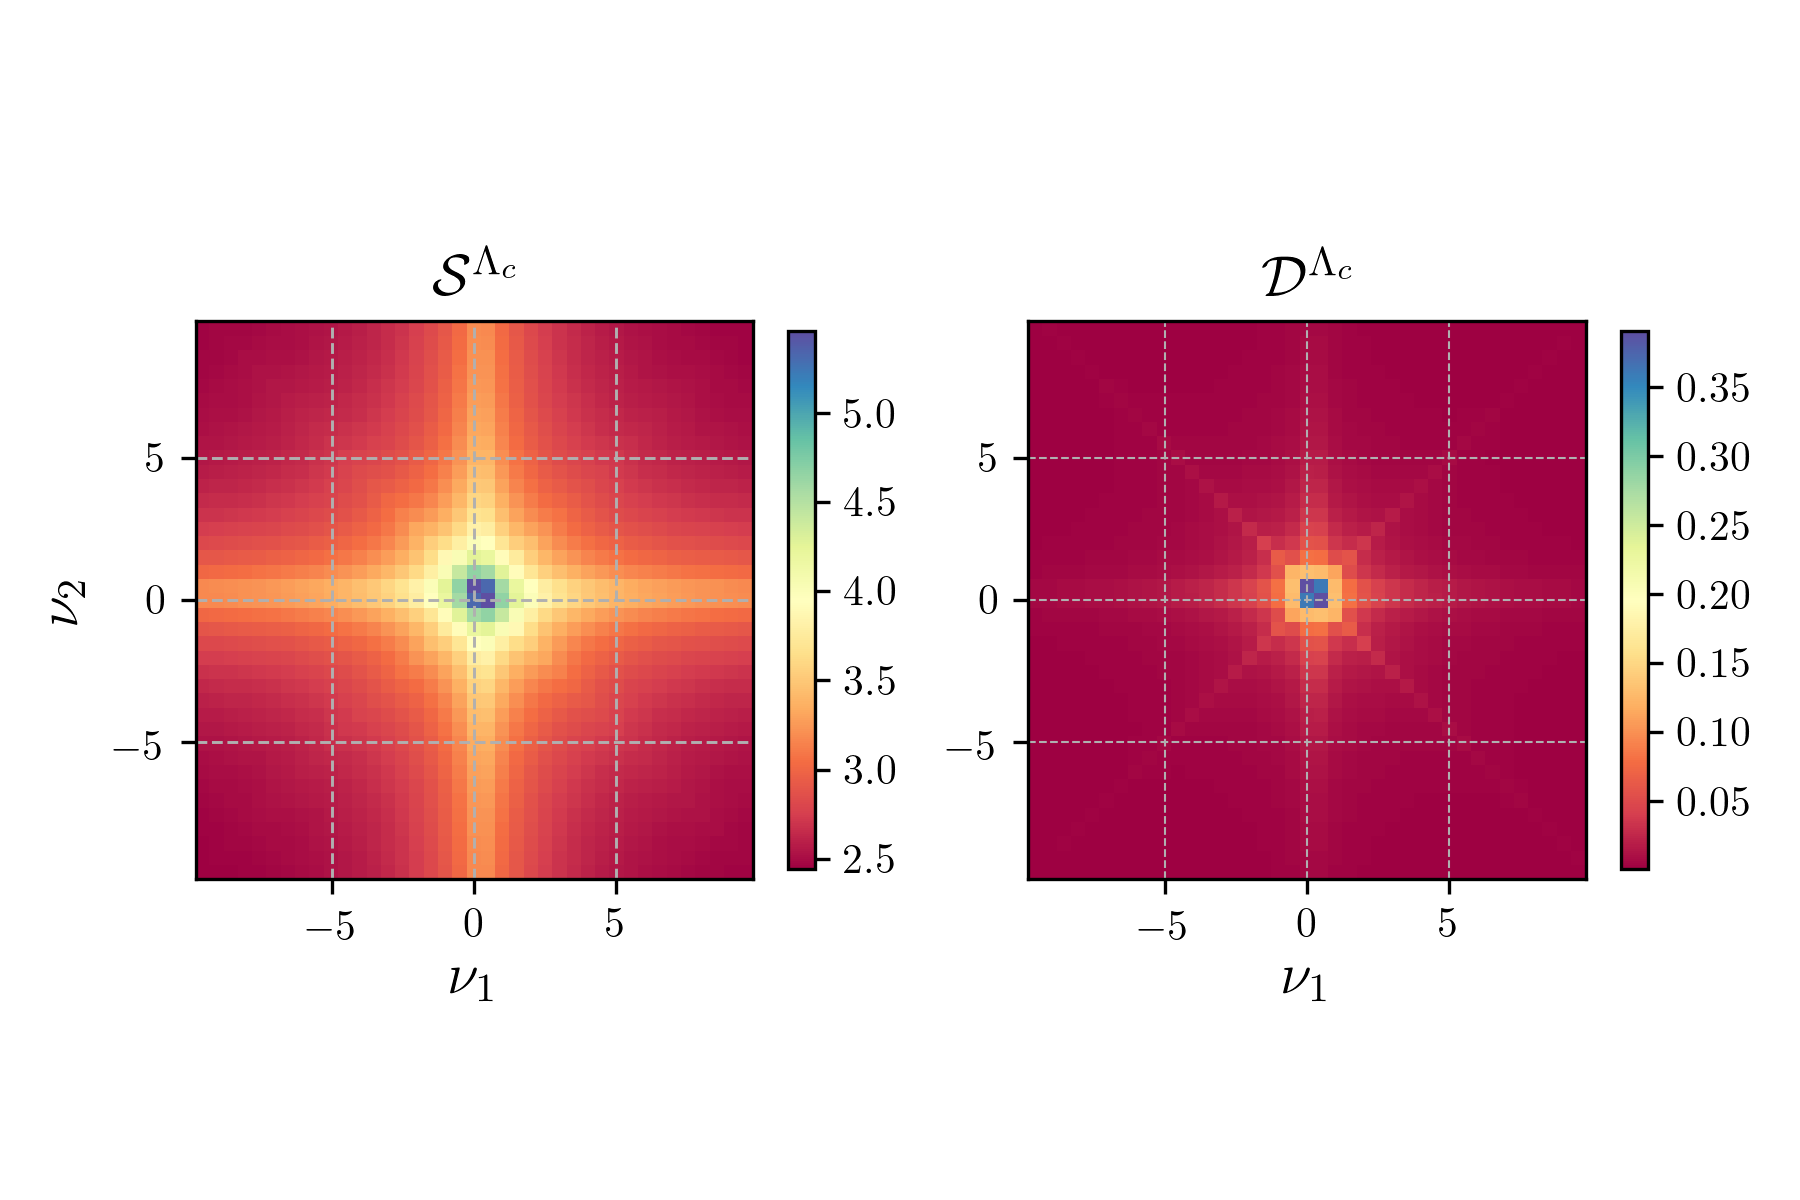
\includegraphics[width=0.60\textwidth]{images/Phi_color_s_d_wave_SE_fill0_975.png}
\caption{Frequency dependence of $\mathcal{S}$ (left panel) and $\mathcal{D}$ (right panel). Here $T=0.08t$, $t'=-0.32t$, $U=4t$ and $x=0.025$. The transfer momentum and frequency are $\bs{Q}=(0,0)$ and $\Omega=0$.}
\label{fig:pairing975}
\end{figure}
\begin{figure}
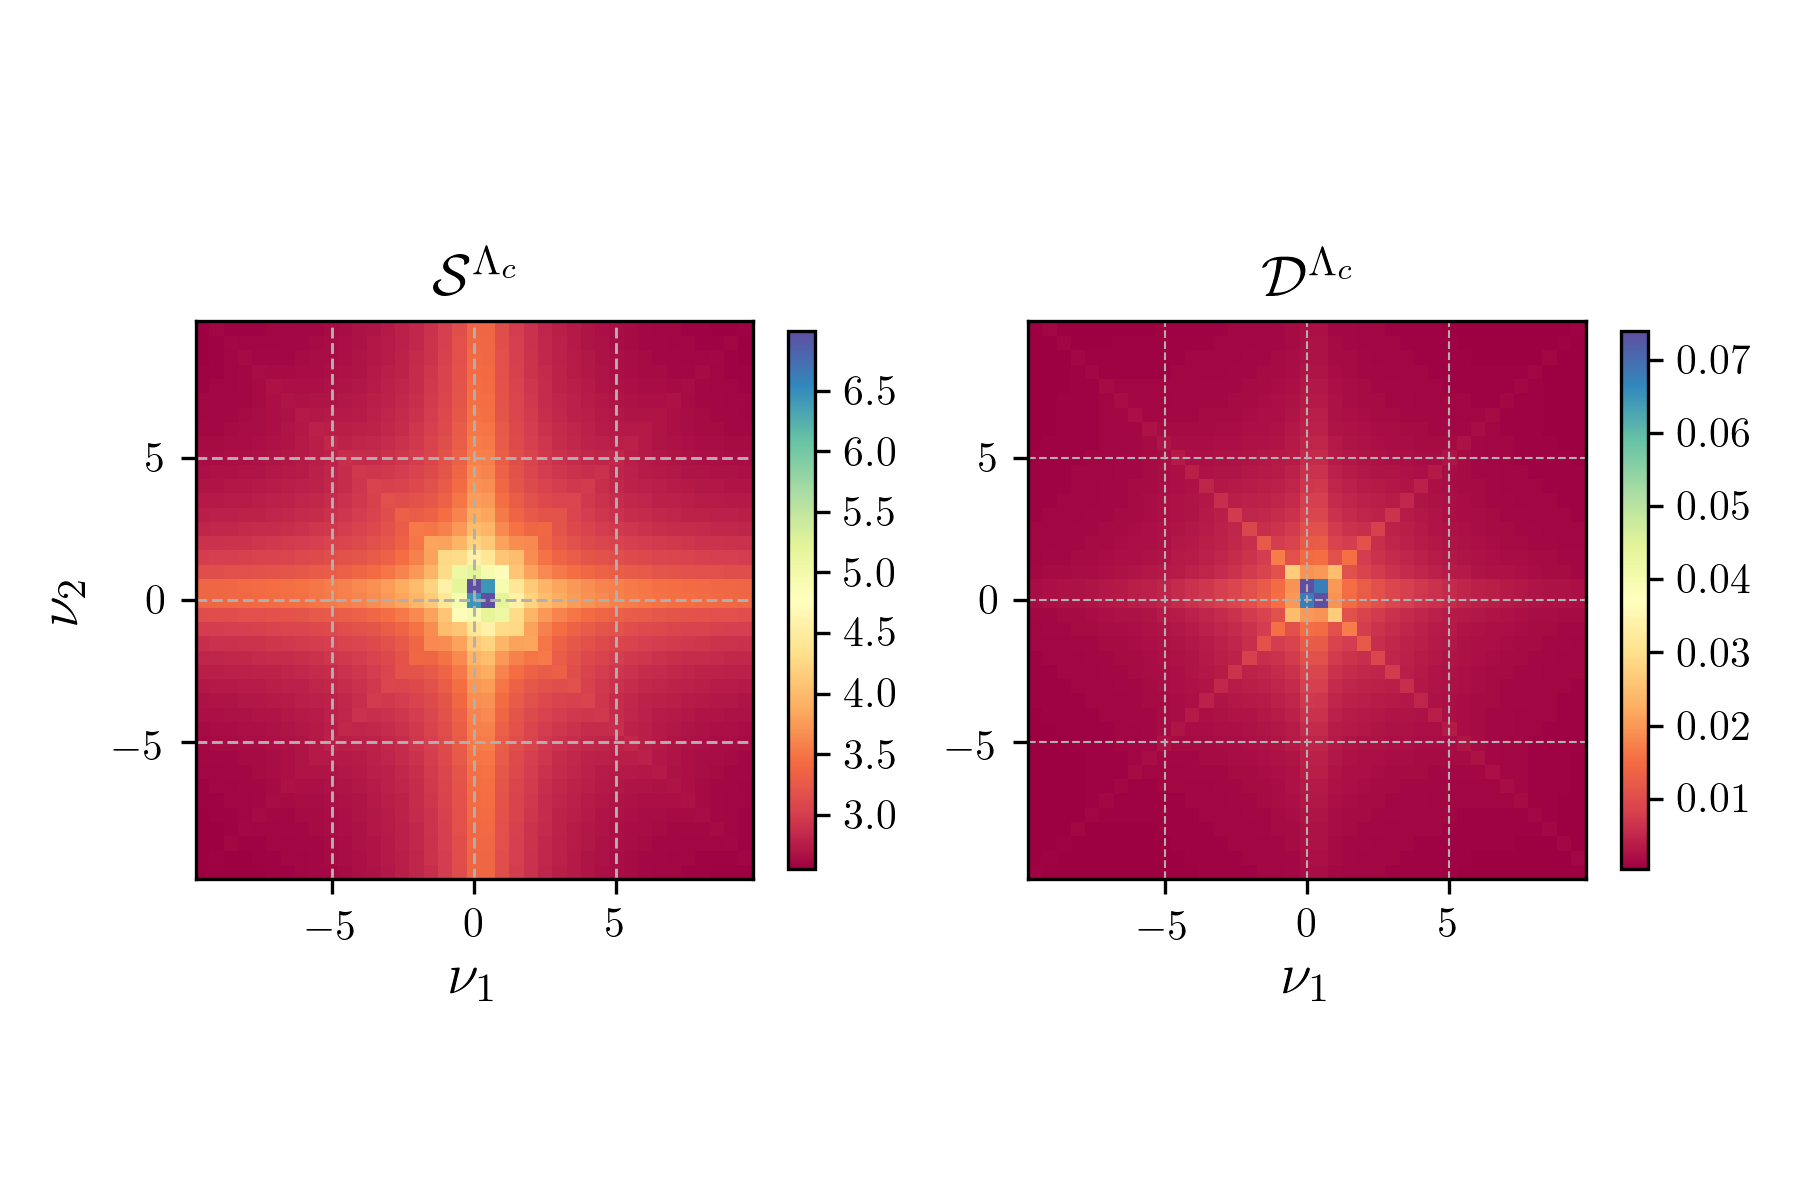
\includegraphics[width=0.60\textwidth]{images/Phi_color_s_d_wave_SE_fill0_600.png}
\caption{Frequency dependence of $\mathcal{S}$ (left panel) and $\mathcal{D}$ (right panel). Here $T=0.08t$, $t'=-0.32t$, $U=4t$ and $x=0.4$. The transfer momentum and frequency are $\bs{Q}=(0,0)$ and $\Omega=0$.}
\label{fig:pairing600}
\end{figure}
In Figs.~\ref{fig:pairing975} and \ref{fig:pairing600} we display the frequency dependence of the pairing functions $\mathcal{S}$ and $\mathcal{D}$. 
As a consequence of Eq.~(\ref{eq:Ldwave}) the frequency structure of $\mathcal{D}$ is decaying in all directions.\cite{Wentzell2016}
The small numerical values are due to three main reasons: 
first, the $d$-wave pairing is expected to increase suddenly for temperatures immediately above its critical temperature. 
Second, as argued in Ref.~\onlinecite{Husemann2012}, previous fRG calculations with a static vertex are likely to overestimate the $d$-wave channel by neglecting the frequency dependence in Eq.~(\ref{eq:Ldwave}). 
Finally, the interaction scheme itself has a tendency to suppress the $d$-wave pairing, since in the terms of Ref.~\onlinecite{Wentzell2016}, its diagrammatic contributions can be classified as \emph{rest function}.
 
